% Options for packages loaded elsewhere
\PassOptionsToPackage{unicode}{hyperref}
\PassOptionsToPackage{hyphens}{url}
\PassOptionsToPackage{dvipsnames,svgnames,x11names}{xcolor}
%
\documentclass[
  12pt]{article}

\usepackage{amsmath,amssymb}
\usepackage{iftex}
\ifPDFTeX
  \usepackage[T1]{fontenc}
  \usepackage[utf8]{inputenc}
  \usepackage{textcomp} % provide euro and other symbols
\else % if luatex or xetex
  \usepackage{unicode-math}
  \defaultfontfeatures{Scale=MatchLowercase}
  \defaultfontfeatures[\rmfamily]{Ligatures=TeX,Scale=1}
\fi
\usepackage{lmodern}
\ifPDFTeX\else  
    % xetex/luatex font selection
\fi
% Use upquote if available, for straight quotes in verbatim environments
\IfFileExists{upquote.sty}{\usepackage{upquote}}{}
\IfFileExists{microtype.sty}{% use microtype if available
  \usepackage[]{microtype}
  \UseMicrotypeSet[protrusion]{basicmath} % disable protrusion for tt fonts
}{}
\makeatletter
\@ifundefined{KOMAClassName}{% if non-KOMA class
  \IfFileExists{parskip.sty}{%
    \usepackage{parskip}
  }{% else
    \setlength{\parindent}{0pt}
    \setlength{\parskip}{6pt plus 2pt minus 1pt}}
}{% if KOMA class
  \KOMAoptions{parskip=half}}
\makeatother
\usepackage{xcolor}
\setlength{\emergencystretch}{3em} % prevent overfull lines
\setcounter{secnumdepth}{5}
% Make \paragraph and \subparagraph free-standing
\ifx\paragraph\undefined\else
  \let\oldparagraph\paragraph
  \renewcommand{\paragraph}[1]{\oldparagraph{#1}\mbox{}}
\fi
\ifx\subparagraph\undefined\else
  \let\oldsubparagraph\subparagraph
  \renewcommand{\subparagraph}[1]{\oldsubparagraph{#1}\mbox{}}
\fi


\providecommand{\tightlist}{%
  \setlength{\itemsep}{0pt}\setlength{\parskip}{0pt}}\usepackage{longtable,booktabs,array}
\usepackage{calc} % for calculating minipage widths
% Correct order of tables after \paragraph or \subparagraph
\usepackage{etoolbox}
\makeatletter
\patchcmd\longtable{\par}{\if@noskipsec\mbox{}\fi\par}{}{}
\makeatother
% Allow footnotes in longtable head/foot
\IfFileExists{footnotehyper.sty}{\usepackage{footnotehyper}}{\usepackage{footnote}}
\makesavenoteenv{longtable}
\usepackage{graphicx}
\makeatletter
\def\maxwidth{\ifdim\Gin@nat@width>\linewidth\linewidth\else\Gin@nat@width\fi}
\def\maxheight{\ifdim\Gin@nat@height>\textheight\textheight\else\Gin@nat@height\fi}
\makeatother
% Scale images if necessary, so that they will not overflow the page
% margins by default, and it is still possible to overwrite the defaults
% using explicit options in \includegraphics[width, height, ...]{}
\setkeys{Gin}{width=\maxwidth,height=\maxheight,keepaspectratio}
% Set default figure placement to htbp
\makeatletter
\def\fps@figure{htbp}
\makeatother

\addtolength{\oddsidemargin}{-.5in}%
\addtolength{\evensidemargin}{-1in}%
\addtolength{\textwidth}{1in}%
\addtolength{\textheight}{1.7in}%
\addtolength{\topmargin}{-1in}%

\makeatletter
\makeatother
\makeatletter
\makeatother
\makeatletter
\@ifpackageloaded{caption}{}{\usepackage{caption}}
\AtBeginDocument{%
\ifdefined\contentsname
  \renewcommand*\contentsname{Table of contents}
\else
  \newcommand\contentsname{Table of contents}
\fi
\ifdefined\listfigurename
  \renewcommand*\listfigurename{List of Figures}
\else
  \newcommand\listfigurename{List of Figures}
\fi
\ifdefined\listtablename
  \renewcommand*\listtablename{List of Tables}
\else
  \newcommand\listtablename{List of Tables}
\fi
\ifdefined\figurename
  \renewcommand*\figurename{Figure}
\else
  \newcommand\figurename{Figure}
\fi
\ifdefined\tablename
  \renewcommand*\tablename{Table}
\else
  \newcommand\tablename{Table}
\fi
}
\@ifpackageloaded{float}{}{\usepackage{float}}
\floatstyle{ruled}
\@ifundefined{c@chapter}{\newfloat{codelisting}{h}{lop}}{\newfloat{codelisting}{h}{lop}[chapter]}
\floatname{codelisting}{Listing}
\newcommand*\listoflistings{\listof{codelisting}{List of Listings}}
\makeatother
\makeatletter
\@ifpackageloaded{caption}{}{\usepackage{caption}}
\@ifpackageloaded{subcaption}{}{\usepackage{subcaption}}
\makeatother
\makeatletter
\@ifpackageloaded{tcolorbox}{}{\usepackage[skins,breakable]{tcolorbox}}
\makeatother
\makeatletter
\@ifundefined{shadecolor}{\definecolor{shadecolor}{rgb}{.97, .97, .97}}
\makeatother
\makeatletter
\makeatother
\makeatletter
\makeatother
\ifLuaTeX
  \usepackage{selnolig}  % disable illegal ligatures
\fi
\usepackage[]{natbib}
\bibliographystyle{agsm}
\IfFileExists{bookmark.sty}{\usepackage{bookmark}}{\usepackage{hyperref}}
\IfFileExists{xurl.sty}{\usepackage{xurl}}{} % add URL line breaks if available
\urlstyle{same} % disable monospaced font for URLs
\hypersetup{
  pdftitle={Visualising How Non-linear Dimension Reduction Warps Your Data},
  pdfauthor={Jayani P.G. Lakshika; Dianne Cook; Paul Harrison; Michael Lydeamore; Thiyanga S. Talagala},
  pdfkeywords={high-dimensional data, dimension
reduction, triangulation, hexagonal binning, low-dimensional
manifold, manifold learning, tour, data vizualization},
  colorlinks=true,
  linkcolor={blue},
  filecolor={Maroon},
  citecolor={Blue},
  urlcolor={Blue},
  pdfcreator={LaTeX via pandoc}}


\begin{document}


\def\spacingset#1{\renewcommand{\baselinestretch}%
{#1}\small\normalsize} \spacingset{1}

%%%%%%%%%%%%%%%%%%%%%%%%%%%%%%%%%%%%%%%%%%%%%%%%%%%%%%%%%%%%%%%%%%%%%%%%%%%%%%

\title{\bf Visualising How Non-linear Dimension Reduction Warps Your
Data}
\author{
Jayani P.G. Lakshika\\
Econometrics \& Business Statistics, Monash University\\
and\\Dianne Cook\\
Econometrics \& Business Statistics, Monash University\\
and\\Paul Harrison\\
MGBP, BDInstitute, Monash University\\
and\\Michael Lydeamore\\
Econometrics \& Business Statistics, Monash University\\
and\\Thiyanga S. Talagala\\
Statistics, University of Sri Jayewardenepura\\
}
\maketitle

\bigskip
\bigskip
\begin{abstract}
Non-Linear Dimension Reduction (NLDR) techniques have emerged as
powerful tools to visualize high-dimensional data. However, their
complexity and parameter choices may lead to distrustful or misleading
results. To address this challenge, we propose a novel approach that
combines the tour technique with a low-dimensional manifold generated
using NLDR techniques, hexagonal binning, and triangulation. This
integration enables a clear examination of the low-dimensional
representation in the original high-dimensional space. Our approach not
only preserves the advantages of both tours and NLDR but also offers a
more intuitive perception of complex data structures and facilitates
accurate data transformation assessments. The method and example data
sets are available in the \textbf{quollr} R package.
\end{abstract}

\noindent%
{\it Keywords:} high-dimensional data, dimension
reduction, triangulation, hexagonal binning, low-dimensional
manifold, manifold learning, tour, data vizualization
\vfill

\newpage
\spacingset{1} % DON'T change the spacing! (Default 1.9)

\ifdefined\Shaded\renewenvironment{Shaded}{\begin{tcolorbox}[interior hidden, breakable, boxrule=0pt, borderline west={3pt}{0pt}{shadecolor}, enhanced, frame hidden, sharp corners]}{\end{tcolorbox}}\fi

\hypertarget{sec-intro}{%
\section{Introduction}\label{sec-intro}}

High-dimensional (high-D) data is widespread in many fields including
ecology and bioinformatics \citep{Guo2023}, in part because of new data
collection technologies \citep{Johnstone2009, ayesha2020overview}.
Working with high-dimensional data poses considerable challenges due to
the difficulty in visualizing beyond two dimensions \citep{Jia2022}.
High-dimensional data also presents difficulties for model fitting
\citep{Johnstone2009}, both computationally and interpretation, each of
which benefits from visualization.

To create visual representations of high-dimensional data, it is common
to apply dimension reduction techniques. Linear methods such as
principal component analysis (PCA) \citep{Karl1901} have been used for
many years, and remain popular. Non-linear methods such as
multi-dimensional scaling (MDS) \citep{Torgerson1967} have also been
routinely used. In the past decade, there has merged many new techniques
non-linear dimension reduction (NLDR), such as t-distributed stochastic
neighbor embedding (tSNE) \citep{Laurens2008}, uniform manifold
approximation and projection (UMAP) \citep{Leland2018}, designed to
capture the complex and non-linear relationships present within
high-dimensional data \citep{Johnstone2009}.

However, projecting high-dimensional data has limitations, such as
information loss and potential distortion of essential structures and
patterns \citep[\citet{article53}]{Jia2022}. The choice of technique and
parameters further impacts the accuracy of the visualization,
necessitating careful consideration for meaningful interpretation (see
Figure~\ref{fig-nldervis}).

Interactive and dynamic graphics systems have also been developed over
the years to enable visualizing high dimensions. One method, called a
tour \citep{Asimov1985}, shows a sequence of linear projections is shown
as a movie, allowing exploration without warping the space
\citep{lee2021review}. Interactive tools like \textbf{XGobi} and
\textbf{GGobi} have been successful in incorporating tours for exploring
high-dimensional data \citep{article60}. The R package \textbf{tourr}
\citep{article61} further enhances tour visualization within R, although
it may face limitations in frame rate and interactive features compared
to \textbf{GGobi}.

To overcome these limitations, the R package \textbf{detourr}
\citep{article22} has been developed, leveraging a Javascript widget via
htmlwidgets \citep{Ramnath2023} to achieve higher frame rates and
enhanced interactivity. Additionally, the R package \textbf{langevitour}
\citep{article09} utilizes Langevin Dynamics to generate a continuous
path of projections, eliminating the need for interpolation between
projections for animation. The tour technique has proven valuable in
exploring statistical model fits \citep{article58} and factorial
experimental designs \citep{article59}. Augmenting the results of
non-linear dimensional reduction methods with the tour, as demonstrated
in the \textbf{liminal} R package \citep{article21}, further enhances
data exploration.

While tours \citep{Asimov1985} preserve space without warping
\citep{lee2021review}, they require integrating multiple low-dimensional
views mentally to perceive high-dimensional structures. To address this
challenge, we propose a novel approach by combining the tour technique
with a low-dimensional manifold. This manifold is created through the
synergistic use of Non-Linear Dimension Reduction (NLDR) techniques,
hexagonal binning, and triangulation. By merging these techniques, our
approach offers a comprehensive and efficient means to visualize and
explore high-dimensional data while retaining the advantages of both
tours and NLDR. This integration facilitates a more intuitive perception
of complex data structures and empowers analysts with a robust tool for
assessing the accuracy of data transformations. The implementation of
our approach is available as an R package called \textbf{quollr}.

The outline of this paper is as follows. The
Section~\ref{sec-background} provides an detailed overview of dimension
reduction methods, triangulation, and tours. Building upon this
foundation, the Section~\ref{sec-methods} delves into the proposed
algorithm, \textbf{quollr}, and its implementation details. In
\textbf{?@sec-prediction}, discusses the effectiveness of the learned
low-dimensional manifold in accurately representing the complex
high-dimensional data. Following that, Section~\ref{sec-simpleex}
presents simple examples from simulations to illustrate the
functionality of the algorithm. Subsequently,
Section~\ref{sec-applications} showcases real-world applications of
\textbf{quollr} on different data sets, particularly in single-cell
RNA-seq data. These applications reveal insights into the performance
and trustworthiness of NLDR algorithms. We analyze the results to
identify situations where NLDR techniques may lead to misleading
interpretations. Finally, \textbf{?@sec-conclusions} concludes by
summarizing the findings and emphasizing the significance of the
proposed approach in tackling the challenges of high-dimensional data
visualization.

\hypertarget{sec-background}{%
\section{Background}\label{sec-background}}

\hypertarget{dimension-reduction}{%
\subsection{Dimension Reduction}\label{dimension-reduction}}

Consider the high-dimensional data a rectangular matrix \(X\), where
\(X = \begin{bmatrix} \textbf{x}_{1} & \textbf{x}_{2} & \cdots & \textbf{x}_{n}\\ \end{bmatrix}\),
with \(n\) observations in \(p\) dimensions. The objective is to
discover a low-dimensional projection
\(Y = \begin{bmatrix} \textbf{y}_{1} & \textbf{y}_{2} & \cdots & \textbf{y}_{n}\\ \end{bmatrix}\),
represented as an \(n\) × \(d\) matrix, where \(d \ll p\). The reduction
process seeks to remove noise from the original data set while retaining
essential information.

There are two main categories of dimension reduction techniques: linear
and non-linear methods. Linear techniques involve a linear
transformation of the data, with one popular example being PCA. PCA
performs an eigen-decomposition of the sample covariance matrix to
obtain orthogonal principal components that capture the variance of the
data \citep{Karl1901}. However, linear methods may not fully capture
complex non-linear relationships present in the data.

In contrast, NLDR techniques generate the low-dimensional representation
\(Y\) from the high-dimensional data \(X\), often using pre-processing
techniques like \(k\)-nearest neighbors graph or kernel transformations.
Multidimensional Scaling (MDS) is a class of NLDR methods that aims to
construct an embedding \(Y\) in a low-dimensional space, approximating
the pair-wise distances in \(X\) \citep{Torgerson1967}. Variants of MDS
include non-metric scaling \citep{article62} and Isomap, which estimate
geodesic distances to create the low-dimensional representation
\citep{article63}. Other approaches based on diffusion processes, like
diffusion maps \citep{article64} and the PHATE algorithm
\citep{article03}, also fall under NLDR methods.

A challenge with NLDR methods is selecting and tuning appropriate
parameters. One specific technique we focus on is Pairwise Controlled
Manifold Approximation (PaCMAP). Similar considerations apply to related
methods like tSNE \citep{Laurens2008}, UMAP \citep{Leland2018}, and
TrMAP \citep{article02}.

It is important to note that methods like PCA and auto-encoders
\citep{article65} provide a reverse mapping from the low-dimensional
space back to the high-dimensional space, enabling data reconstruction.
However, many non-linear methods, including tSNE, prioritize
visualization and exploration over reconstruction. Their focus is on
capturing complex structures that may not be easily represented in the
original space, making a straightforward reverse mapping challenging.

\hypertarget{non-linear-dimension-reduction-techniques}{%
\subsubsection{Non-linear dimension reduction
techniques}\label{non-linear-dimension-reduction-techniques}}

Non-linear dimension reduction techniques play a crucial role in the
analysis and visualization of high-dimensional data, where the
complexities of relationships among variables may not be adequately
captured by linear methods. Among these techniques, tSNE stands out for
its emphasis on preserving pairwise distances. By minimizing the
divergence between probability distributions in both the high and
low-dimensional spaces, t-SNE effectively reveals intricate structures
and patterns within the data. Its application is widespread in tasks
requiring the visualization of clusters and local relationships, though
it does require careful consideration of the perplexity parameter for
optimal results.

UMAP is another powerful non-linear technique that strikes a balance
between preserving local and global structures. Constructing a fuzzy
topological representation using a weighted k-nearest neighbors graph,
UMAP optimizes the low-dimensional embedding to resemble this
representation. Known for its efficiency and scalability, UMAP is
versatile across various scales of relationships in the data, although
parameter sensitivity, particularly concerning the choice of neighbors,
must be taken into account.

For trajectory data, PHATE provides specialized capabilities. It models
the affinity between data points, simulating a heat diffusion process to
capture developmental processes, particularly in single-cell genomics.
While PHATE excels in revealing trajectory structures and offering
insights into cellular development, it necessitates careful parameter
tuning due to its specialized nature.

TriMAP adopts a unique approach by approximating the data manifold
through the construction of a triangulated graph representation. This
technique efficiently captures both global and local structures by
representing the data as a network of triangles. TriMAP's strength lies
in its ability to efficiently capture complex structures, albeit with
sensitivity to parameter choices, including the number of neighbors.

In contrast, PaCMAP introduces supervised learning to create a
low-dimensional representation while preserving pair-wise relationships.
Constructing a graph based on pair-wise distances, PaCMAP optimizes an
embedding using a customizable loss function. Particularly notable is
PaCMAP's flexibility in incorporating class labels or additional
information to guide the embedding process, offering users a means to
customize its behavior and performance.

\begin{figure}

{\centering 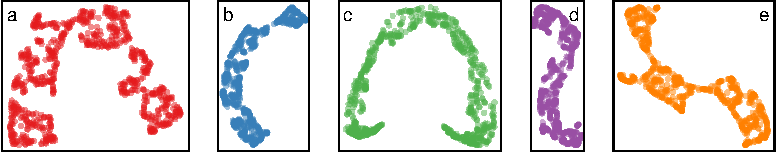
\includegraphics[width=1\textwidth,height=\textheight]{paper_files/figure-pdf/fig-nldervis-1.pdf}

}

\caption{\label{fig-nldervis}2D layouts from different NLDR techniques
applied the same data: (a) tSNE (perplexity = 27), (b) UMAP
(n\_neighbors = 50), (c) PHATE (knn = 5), (d) TriMAP (n\_inliers = 5,
n\_outliers = 4, n\_random = 3), and (e) PaCMAP (n\_neighbors = 10, init
= random, MN\_ratio = 0.9, FP\_ratio = 2). Is there a best
representation of the original data or are they all providing equivalent
information?}

\end{figure}

\hypertarget{linear-overviews-using-tours}{%
\subsection{Linear overviews using
tours}\label{linear-overviews-using-tours}}

A tour is a powerful visualization technique used to explore
high-dimensional data by generating a sequence of projections, typically
into two dimensions. There are two main types of tours: the Grand Tour
and the Guided Tour. The Grand Tour explores the data's shape and global
structure by using random projections \citep{Asimov1985}. In contrast,
the Guided Tour focuses on specific patterns by moving towards
interesting projections defined by a predefined index function
\citep{article29}.

The process begins with a real data matrix \(X\) containing \(n\)
observations in \(p\) dimensions. It generates a sequence of \(p\) ×
\(d\) orthonormal projection matrices (bases), usually 1 or 2
dimensions. For each pair of orthonormal bases \(A_t\) and \(A_{t+1}\),
a geodesic path is interpolated to create smooth animation between
projections.

In the Grand Tour, new orthonormal bases are randomly chosen to explore
the \(d\)-dimensional subspace. The data is often sphered via principal
components to reduce dimensionality. The Guided Tour uses a predefined
index function to generate a sequence of `interesting' projections. The
resulting tour continuously visualizes the projected data \(Y_t\) =
\(XA_t\) as it interpolates between successive bases.

While both tours can be used to visualize data, examples often focus on
using the Grand Tour to observe global structures. However, software
like \textbf{langevitour} can visualize both types of tours, providing
flexibility for exploring high-dimensional data with various objectives.

\hypertarget{sec-methods}{%
\section{Methodology}\label{sec-methods}}

Our algorithm comprises two main phases: (1) generate the model in the
2D space, and (2) generate the model in the high-D space. These two
phases are described in details in this section.

\begin{figure}

{\centering 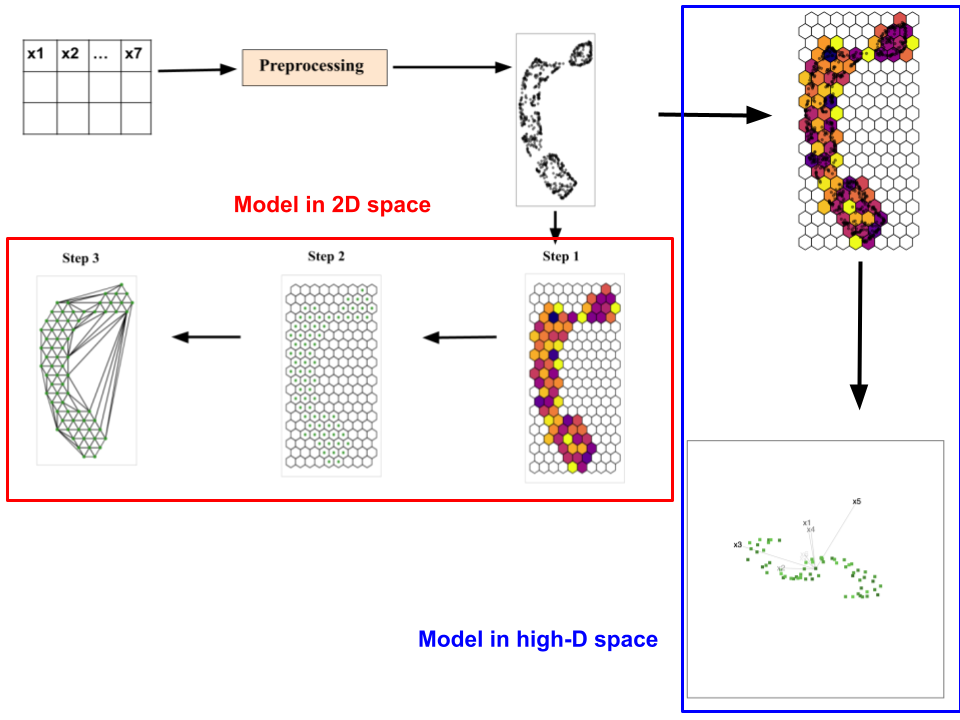
\includegraphics[width=1\textwidth,height=1\textheight]{figures/workflow.png}

}

\caption{\label{fig-meth}A flow diagram detailing the steps taken to
create the low-dimensional manifold in the high dimensional space. There
are two basic phases, one to generate the model in the 2D space, and
other to generate the model in the high-D space.}

\end{figure}

\hypertarget{preprocessing-steps}{%
\subsection{Preprocessing steps}\label{preprocessing-steps}}

To tackle the complexities and noise in high-dimensional data, we apply
PCA as a pre-processing step \citep[\citet{article68},
\citet{article69}]{article67}. This step helps in noise reduction by
identifying principal components that represent directions of maximum
variance, capturing essential patterns in the data.

\hypertarget{constructing-the-2d-model}{%
\subsection{Constructing the 2D model}\label{constructing-the-2d-model}}

\textbf{Step 1: Computing the hexagonal grid configuration}

Hexagonal binning is a data visualization technique that aggregates
high-dimensional data into a two-dimensional representation using
hexagonal regions called bins \citep{article66}. The hexagonal shape is
preferred due to its circular-like appearance, providing smoother
transitions between neighboring bins and efficient data aggregation.
This technique is especially useful for handling large data sets as it
reduces visual clutter while capturing the underlying data distribution
effectively. By considering the data distribution, important features
are captured, and gaps between bins are minimized, leading to a more
accurate representation of the data. In our algorithm, hexagonal binning
is utilized to create a low-dimensional manifold.

\textbf{(a) Determine the number of bins along the x-axis} (\(b_1\))

The first step involves to determine the optimal number of bins (\(b\))
for creating regular hexagons in the hexagonal grid. To achieve this, we
rely on the relationship between the diameter (\(h\)) and the area
(\(A\)) of regular hexagons, as given by Equation~\ref{eq-equation3}.

\begin{equation}\protect\hypertarget{eq-equation3}{}{
 \text{A} = \frac{\sqrt{3}}{2}h^2
}\label{eq-equation3}\end{equation}

To capture the data's structure effectively, we consider the optimal
\(A = 1\) (see Figure~\ref{fig-binsize}). Using
Equation~\ref{eq-equation4}, we then calculate \(h\) of a regular
hexagon.

\begin{equation}\protect\hypertarget{eq-equation4}{}{
  \text{h} = \sqrt{\frac{2}{\sqrt{3}}A}
}\label{eq-equation4}\end{equation}

Next, we refer the \texttt{hexbin} function in R, which provides a
relationship between the diameter of the hexagon (\(h\)) and the number
of bins along the x-axis (\(b_1\)) (Equation~\ref{eq-equation6}).

\begin{equation}\protect\hypertarget{eq-equation6}{}{
h = \frac{r_1}{b_1}
}\label{eq-equation6}\end{equation}

By utilizing the calculated \(h\) and the range of the non-linear
projection component 1 (\(r_1\)), we determine the \(b_1\)
(Equation~\ref{eq-equation5}). The result is rounded up to the nearest
whole number to ensure an appropriate number of bins that capture the
variability of the data along the x-axis.

\begin{equation}\protect\hypertarget{eq-equation5}{}{
b_1 = \frac{r_1}{h}
}\label{eq-equation5}\end{equation}

\textbf{(b) Determine the effective shape parameter} (\(s\))

In this step, we determine the optimal shape parameter (\(s\)) for the
hexagonal bins, which significantly influences their shape and
arrangement within the grid. The shape parameter (\(s\)) in the
hexagonal binning algorithm is defined as the ratio of the height
(\(y\)) to the width (\(x\)) of the plotting region, referring to the
\texttt{hexbin} function in R (see Equation~\ref{eq-equation1}). It
determines the shape of the plotting regions and plays a vital role in
generating an appropriate hexagonal grid for the data visualization.

\begin{equation}\protect\hypertarget{eq-equation1}{}{
s = \frac{y}{x}
}\label{eq-equation1}\end{equation}

To calculate the effective shape parameter (\(s\)) for our algorithm, we
consider the ranges of the non-linear projection components. Denoting
the range of the non-linear projection component 1 as \(r_1\) and the
range of the non-linear projection component 2 as \(r_2\), we find the
shape parameter using Equation~\ref{eq-equation2}.

\begin{equation}\protect\hypertarget{eq-equation2}{}{
s = \frac{r_2}{r_1}
}\label{eq-equation2}\end{equation}

\begin{figure}[H]

{\centering 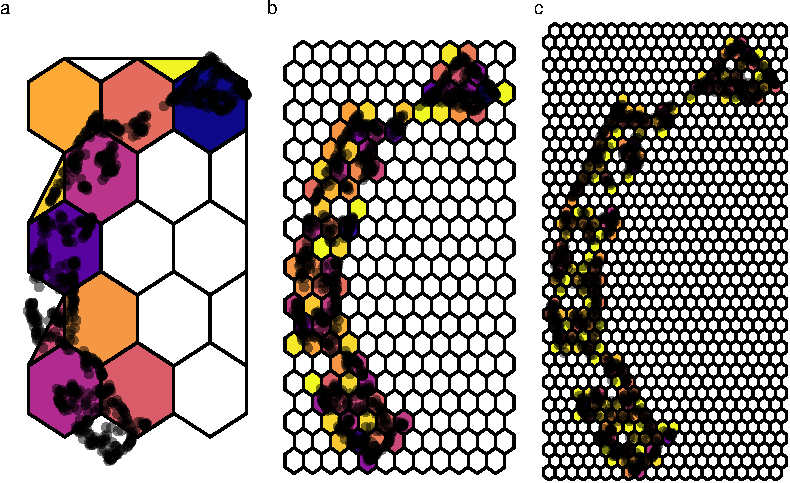
\includegraphics{paper_files/figure-pdf/fig-binsize-1.pdf}

}

\caption{\label{fig-binsize}Hexbin plots from different number of bins
for the same \textbf{s\_curve\_noise\_umap} data: (a) b = (4, 8), s =
1.643542, (b) b = (12, 22), s = 1.643542, and (c) b = (21, 40), s =
1.643542. The hexbins are colored based on the density of points, with
yellow indicating higher point density and darker colors representing
lower point density within each bin. Does a value of number of bins
exist to effectively represent the low-dimensional data?}

\end{figure}

\textbf{Step 2: Obtain bin centroids}

After computing hexagonal grid configurations, the 2D emdeddings are
binned into hexagon cells. As a result of hexagonal binning , the bin
centroids (\(C_k^{(2)} \equiv (C_{kx}, C_{ky}\))) (see
Figure~\ref{fig-meth} (Step 2)) are obtained.

\textbf{Step 3: Triangulate bin centroids}

In this step, the algorithm proceeds to triangulate the centroids (see
Figure~\ref{fig-meth} (Step 3)) of the hex bins. Triangulation is a
fundamental process in computational geometry and computer graphics that
involves dividing a set of points in a given space into interconnected
triangles \citep{article30}. One common algorithm used for triangulation
is Delaunay triangulation \citep{article26}, where points are connected
in a way that maximizes the minimum angles of the resulting triangles,
leading to a more regular and well-conditioned triangulation. In our
algorithm, triangulation helps us identify geometric relationships and
patterns in the data.

Since we are working with the centroids of regular hexagonal bins, the
resulting mesh will predominantly comprise equal-sized regular
triangles. However, the triangulation also helps span any gaps that may
exist between clusters of points, allowing for a more complete and
interconnected representation of the data.

\hypertarget{lifting-the-model-into-high-dimensions}{%
\subsection{Lifting the model into high
dimensions}\label{lifting-the-model-into-high-dimensions}}

Creating the model in the high-D space involves a two-step process.
Initially, we identify observations within each hexagonal bin. After
this, we calculate the average of the high-dimensional data within each
hex bin. The resulting values represent the averaged high-dimensional
data points (\(C_k^{(p)} \equiv (C_{kx_1}, ..., C_{kx_p}\))).
Essentially, these averaged high-dimensional data points serve as the
representation of the hex bin centroids in the high-D space.

\begin{figure}

{\centering 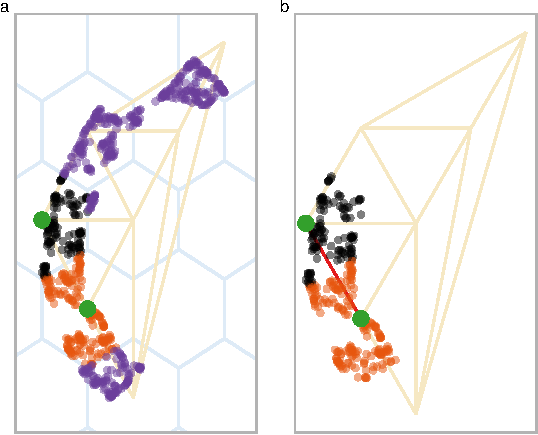
\includegraphics{paper_files/figure-pdf/fig-wkhighD-1.pdf}

}

\caption{\label{fig-wkhighD}How the 2D model lift into high dimensions?
(a) visualize the points and the hexagonal bin centroids related 2nd and
15th hexagons, (b) visualization of the edge connected the 2nd and 15th
hexagons (colored in red) in the triangular mesh. A video of tour
animation is available at
\url{https://www.youtube.com/watch?v=vBvM30Plt24}.}

\end{figure}

\hypertarget{tunning-the-model}{%
\subsection{Tunning the model}\label{tunning-the-model}}

In our model tuning process, we strategically adjust three key
parameters to optimize the performance and accuracy of our approach.
They are (i) the total number of bins (\(b\)), (ii) a benchmark value to
remove low-density hexagons, and (iii) a benchmark value to remove long
edges.

\hypertarget{total-number-of-bins}{%
\subsubsection{Total number of bins}\label{total-number-of-bins}}

The total number of bins is a crucial parameter that defines the
granularity of our hexagonal grid. This parameter particularly
influential in capturing the intricacies of the data structure. It is
determined by multiplying the number of bins along the x-axis ((b\_1))
with the number of bins along the y-axis ((b\_2)), as per the formula:

\begin{equation}\protect\hypertarget{eq-equationp1}{}{
b = b_1 \times b_2
}\label{eq-equationp1}\end{equation}

Here, (b) represents the total number of bins. Adjusting the parameter
(b\_1) provides control over the total bin count ((b)), allowing us to
fine-tune the grid's configuration along the x-axis based on specific
requirements.

\hypertarget{benchmark-value-to-remove-low-density-hexagons}{%
\subsubsection{Benchmark value to remove low-density
hexagons}\label{benchmark-value-to-remove-low-density-hexagons}}

Addressing low-density hexagons is a systematic process to handle
sparsely represented data in certain regions. For each hex bin, we
identify the six nearest hex bins using an equal 2D distance metric.
Then, we calculate the mean density, as outlined in the equations:

\begin{equation}\protect\hypertarget{eq-equationp2}{}{
\text{standard count} = \frac{\text{count}}{\text{max count}} 
}\label{eq-equationp2}\end{equation}

\begin{equation}\protect\hypertarget{eq-equationp3}{}{
\text{mean density} = \frac{\text{standard count}}{6} 
}\label{eq-equationp3}\end{equation}

The standard count is derived from the number of observations in the hex
bins. By examining the distribution of mean densities and designating
the first quartile as the benchmark value, hex bins with mean densities
below this benchmark are removed. This process ensures the elimination
of regions with insufficient data density, focusing on areas with more
significant data representation and preserving the overall structure in
the low-dimensional space.

\hypertarget{benchmark-value-to-remove-long-edges}{%
\subsubsection{Benchmark value to remove long
edges}\label{benchmark-value-to-remove-long-edges}}

The removal of long edges is a critical step to create a smoother
representation by iteratively eliminating hexagons with excessive
distances between centroids. This process eliminates outliers and noise
while preserving essential local relationships within the data. To
achieve this, distances between vertices are sorted, and unique distance
values are extracted. By setting a threshold based on the largest
difference between consecutive distance values, long edges are
identified and removed. This refinement step contributes to enhancing
the quality of the triangular mesh, ensuring a more accurate
representation of the data structure.

\hypertarget{sec-summary}{%
\subsection{Model summaries}\label{sec-summary}}

\hypertarget{predicted-values-and-residuals}{%
\subsubsection{Predicted values and
residuals}\label{predicted-values-and-residuals}}

In this context, the term ``prediction values'' refers to the 2D
coordinates predicted for the NLDR technique. The approach involves
employing the K-nearest neighbors (KNN) algorithm to identify the
nearest hexagonal bin centroid in the 2D space. Subsequently, the
coordinates of this centroid are assigned as the low-dimensional
predicted values for the test data in 2D space. It is noteworthy that
traditional NLDR methods, such as t-SNE, often lack a direct predict
function, making our approach valuable for generating predicted values
in the absence of such functionalities.

The concept of ``residuals'' is pivotal in evaluating the accuracy of
representing bin centroids in high dimensions. To quantify this
accuracy, we introduce an error metric, which measures the sum of
squared differences between the high-dimensional data (\(x_{ij}\)) and
the predicted bin centroid data in high-dimensional space (\(C_{x_ij}\))
across all bins and dimensions. Mathematically, this error is expressed
as:

\begin{equation}\protect\hypertarget{eq-equation11}{}{
\text{Error} = \sum_{j = 1}^{n}\sum_{i = 1}^{p} (x_{ij} - C_{x_ij})^2
}\label{eq-equation11}\end{equation}

Here, \(n\) represents the number of bins, \(p\) represents the
dimensions, \(x_{ij}\) is the actual high-dimensional data, and
\(C_{x_ij}\) is the predicted bin centroid data in high dimensions.

The error metric outlined above provides valuable insights into the
overall accuracy of our predictive model. By quantifying the squared
deviations between the actual and predicted values across all bins and
dimensions, we gain a comprehensive understanding of how well our method
captures and represents the underlying structure of the data in the
reduced 2D space. This assessment is crucial for evaluating the efficacy
of our NLDR technique in preserving the essential information present in
the original high-dimensional data.

\hypertarget{goodness-of-fit-statistics}{%
\subsubsection{Goodness of fit
statistics}\label{goodness-of-fit-statistics}}

Moving on to the assessment of prediction accuracy, we calculate the
Mean Squared Error (MSE). The MSE helps measure the average squared
differences between the actual high-dimensional data (\(x_{ij}\)) and
the predicted bin centroid data in high-D (\(C_{x_ij}\)) values across
all bins. Mathematically, this is expressed as:

\begin{equation}\protect\hypertarget{eq-equation9}{}{
\text{MSE} = \sum_{j = 1}^{n} \frac{\sum_{i = 1}^{p} (x_{ij} - C_{x_ij})^2}{\text{total number of bins}}
}\label{eq-equation9}\end{equation}

Here, \(b\) signifies the total number of bins, \(p\) denotes the number
of dimensions in the high-dimensional data, and \(n\) represents the
number of observations.

Additionally, we gauge the model's performance using the Akaike
Information Criterion (AIC), calculated by the formula:

\begin{equation}\protect\hypertarget{eq-equation10}{}{
\text{AIC} = 2bp + np * log(\text{MSE})
}\label{eq-equation10}\end{equation}

These metrics, MSE and AIC, collectively offer valuable insights into
the model's predictive performance, considering both accuracy and
complexity in the predictions.

\begin{figure}

{\centering 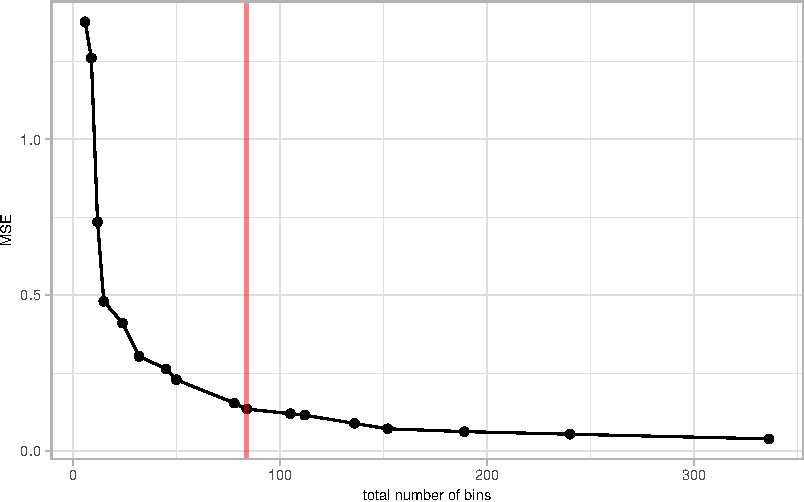
\includegraphics[width=1\textwidth,height=\textheight]{paper_files/figure-pdf/fig-diagnosticpltScurve-1.pdf}

}

\caption{\label{fig-diagnosticpltScurve}Goodness of fit statistics from
different NLDR techniques applied to training S-curve dataset. What is
the best NLDR technique to represent the original data in 2D?}

\end{figure}

\begin{figure}

{\centering 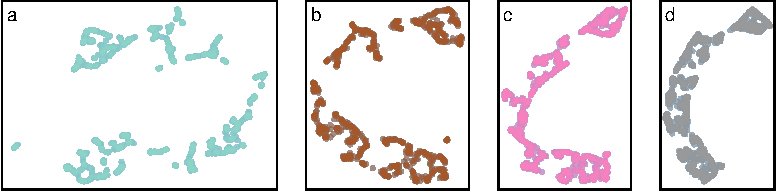
\includegraphics[width=1\textwidth,height=\textheight]{paper_files/figure-pdf/fig-nldervisUMAP-1.pdf}

}

\caption{\label{fig-nldervisUMAP}2D layouts from UMAP applied for the
S-curve data: (a) UMAP (n\_neighbors = 7), (b) UMAP (n\_neighbors = 15),
(c) UMAP (n\_neighbors = 32), (d) UMAP (n\_neighbors = 50). Is there a
best parameter choice in representing UMAP or are they all providing
equivalent information?}

\end{figure}

\begin{figure}

{\centering 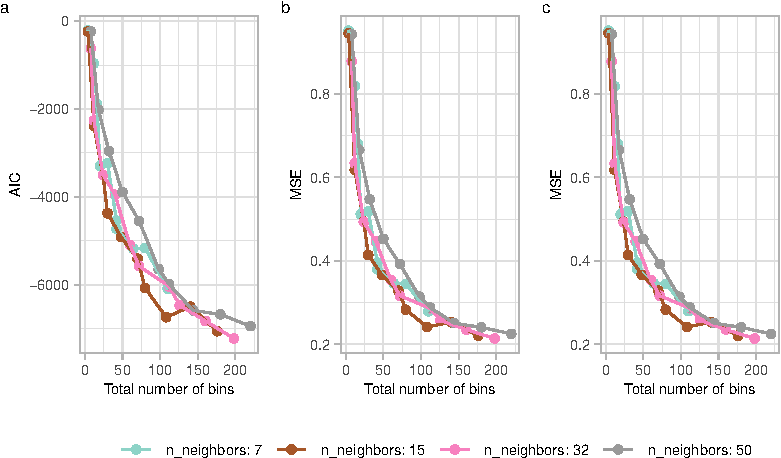
\includegraphics[width=1\textwidth,height=\textheight]{paper_files/figure-pdf/fig-diagnosticpltDiffParam-1.pdf}

}

\caption{\label{fig-diagnosticpltDiffParam}Goodness of fit statistics
from different n\_neighbors parameter of UMAP applied to training
S-curve dataset. What is the best parameter choice in UMAP to represent
the original data in 2D?}

\end{figure}

\hypertarget{sec-simpleex}{%
\subsection{Simulated data example}\label{sec-simpleex}}

In this section, we showcase the effectiveness of our methodology using
simulated data. The dataset comprises five spherical Gaussian clusters
in 4-\(d\), with each cluster containing an equal number of points and
consistent within variation.

We \emph{strongly} recommend viewing the linked videos for each study
while reading. Links to the videos are available in the figures for each
example. The videos show the visual appearance of the
\textbf{langevitour} interface with low-dimensional view and how we can
interact with the tour via the controls.

\begin{figure}

{\centering 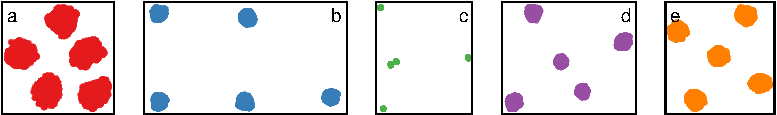
\includegraphics[width=1\textwidth,height=\textheight]{paper_files/figure-pdf/fig-nldervis5Gau-1.pdf}

}

\caption{\label{fig-nldervis5Gau}2D layouts from different NLDR
techniques applied the same data: (a) tSNE (perplexity = 61), (b) UMAP
(n\_neighbors = 15), (c) PHATE (knn = 5), (d) TriMAP (n\_inliers = 5,
n\_outliers = 4, n\_random = 3), and (e) PaCMAP (n\_neighbors = 10, init
= random, MN\_ratio = 0.9, FP\_ratio = 2). Is there a best
representation of the original data or are they all providing equivalent
information?}

\end{figure}

\begin{figure}

{\centering 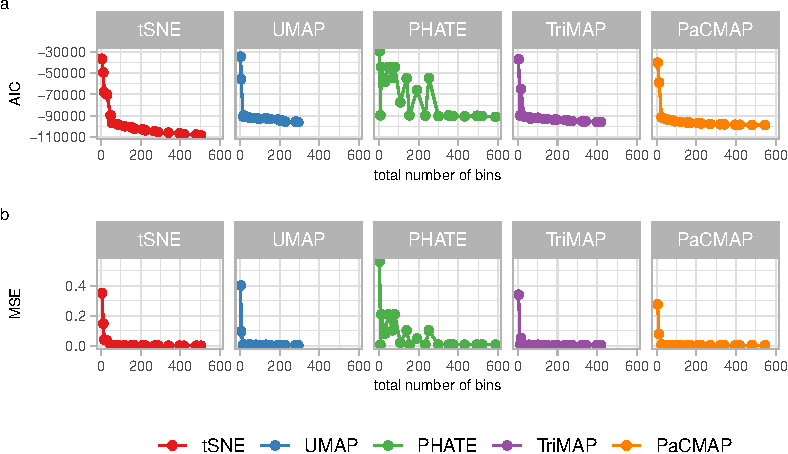
\includegraphics[width=1\textwidth,height=\textheight]{paper_files/figure-pdf/fig-diagnosticpltGau-1.pdf}

}

\caption{\label{fig-diagnosticpltGau}Goodness of fit statistics from
different NLDR techniques applied to training five spherical Gaussian
cluster dataset. What is the best NLDR technique to represent the
original data in 2D?}

\end{figure}

\hypertarget{sec-applications}{%
\section{Applications}\label{sec-applications}}

\hypertarget{single-cell-rna-seq-data-of-human}{%
\subsection{Single-cell RNA-seq data of
human}\label{single-cell-rna-seq-data-of-human}}

In the field of single-cell studies, a common analysis task involves
clustering to identify groups of cells with similar expression profiles.
Analysts often turn to NLDR techniques to verify and identify these
clusters and explore developmental trajectories (e.g., example 1). In
clustering workflows, the main objective is to verify the existence of
clusters and subsequently identify them as specific cell types by
examining the expression of ``known'' marker genes. In this context, a
``faithful'' embedding should ideally preserve the topology of the data,
ensuring that cells corresponding to the same cell type are situated
close to the high-dimensional space.

To begin our analysis, we installed the Peripheral Blood Mononuclear
Cells (pbmc) data set obtained from 10x Genomics using the
\texttt{SeuratData} R package \citep{Rahul2019}, which facilitates the
distribution of data sets in the form of Seurat objects
\citep{Yuhan2021}. This data set contains 13,714 features across 2,700
samples within a single assay. The active assay is RNA, with 13,714
features representing different gene expressions. After loading the data
set, we obtained the principal components (PCs) and assessed the
variance explained by each PC. Based on this evaluation, we selected
seven PCs, representing approximately 50\% of the variance in gene
expression, for further analysis.

Next, we employed the UMAP technique with default parameter settings. As
illustrated in \textbf{?@fig-pbmc}, the cell types B and Platelet are
well-separated in the UMAP layout. Moreover, CD14+ Mono, FCGR3A+ Mono,
and DC form a distinct cluster, while Naive CD4 T, NK, Memory CD4 T, and
CD8 T are grouped together in another cluster. The values utilized to
construct the smooth low-dimensional manifold are presented in
\textbf{?@tbl-table02}. The linked video, demonstrating the tour with
the model, showcases the generation of a smooth surface for this
application, enabling a comprehensive exploration of the data's
structure and relationships (see \textbf{?@fig-pbmc\_sc}).

\begin{figure}

{\centering 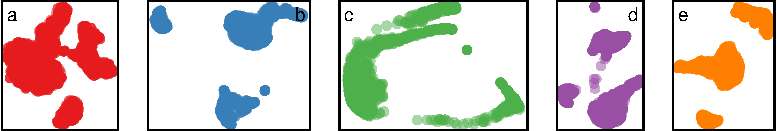
\includegraphics[width=1\textwidth,height=\textheight]{paper_files/figure-pdf/fig-nldervis5PBMC-1.pdf}

}

\caption{\label{fig-nldervis5PBMC}2D layouts from different NLDR
techniques applied for the training PBMC dataset: (a) tSNE (perplexity =
30), (b) UMAP (n\_neighbors = 15), (c) PHATE (knn = 5), (d) TriMAP
(n\_inliers = 5, n\_outliers = 4, n\_random = 3), and (e) PaCMAP
(n\_neighbors = 10, init = random, MN\_ratio = 0.9, FP\_ratio = 2). Is
there a best representation of the original data or are they all
providing equivalent information?}

\end{figure}

\begin{figure}

{\centering 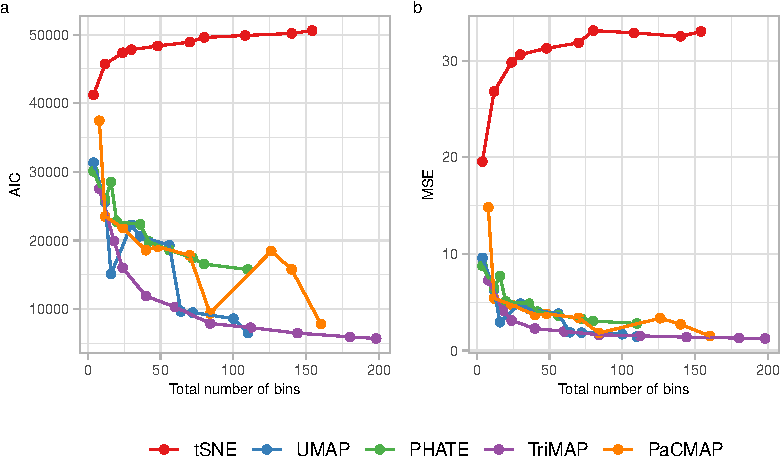
\includegraphics[width=1\textwidth,height=\textheight]{paper_files/figure-pdf/fig-diagnosticpltPBMC-1.pdf}

}

\caption{\label{fig-diagnosticpltPBMC}Goodness of fit statistics from
different NLDR techniques applied to training PBMC dataset. What is the
best NLDR technique to represent the original data in 2D?}

\end{figure}

\hypertarget{single-cell-tagged-reverse-transcription-sequencing-data-of-mouse}{%
\subsection{Single-Cell Tagged Reverse Transcription sequencing data of
mouse}\label{single-cell-tagged-reverse-transcription-sequencing-data-of-mouse}}

The Zeisel mouse brain dataset, obtained through Spatial Transcriptomics
(STRT-Seq). Within this dataset, information is collected from a
substantial 2,816 individual mouse brain cells. Each of these cells acts
as a molecular snapshot, capturing the distinctive genetic activity
within various cell types. This diversity spans neurons, glial cells,
and other essential components of the brain, offering a comprehensive
view of the cellular tapestry.

What makes this dataset particularly valuable is its ability to shed
light on the spatial distribution of cells. Researchers can explore how
gene expression patterns vary across different regions of the mouse
brain, unlocking insights into the functional specialization of these
regions and the intricate networks that underpin neural processes.

\begin{figure}

{\centering 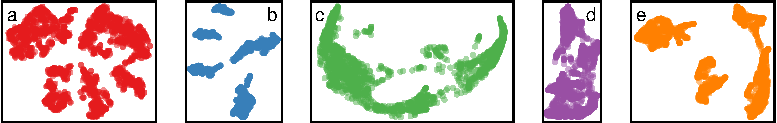
\includegraphics[width=1\textwidth,height=\textheight]{paper_files/figure-pdf/fig-nldervis5Mouse-1.pdf}

}

\caption{\label{fig-nldervis5Mouse}2D layouts from different NLDR
techniques applied for the training Zeisel mouse brain dataset: (a) tSNE
(perplexity = 30), (b) UMAP (n\_neighbors = 15), (c) PHATE (knn = 5),
(d) TriMAP (n\_inliers = 5, n\_outliers = 4, n\_random = 3), and (e)
PaCMAP (n\_neighbors = 10, init = random, MN\_ratio = 0.9, FP\_ratio =
2). Is there a best representation of the original data or are they all
providing equivalent information?}

\end{figure}

\begin{figure}

{\centering 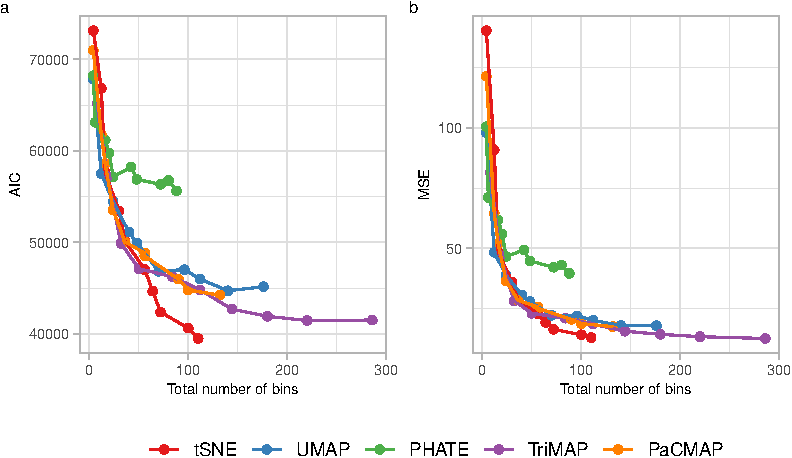
\includegraphics[width=1\textwidth,height=\textheight]{paper_files/figure-pdf/fig-diagnosticpltZEI-1.pdf}

}

\caption{\label{fig-diagnosticpltZEI}Goodness of fit statistics from
different NLDR techniques applied to training Zeisel mouse brain
dataset. What is the best NLDR technique to represent the original data
in 2D?}

\end{figure}

\hypertarget{sec-discussion}{%
\section{Discussion}\label{sec-discussion}}

Our research introduces a comprehensive framework that leverages tours
for interactive exploration of high-dimensional data coupled with a
low-dimensional manifold, facilitated by the \texttt{quollr} R package.
Regardless of the Non-Linear Dimension Reduction (NLDR) technique in
use, our approach demonstrates effectiveness through simulation
examples, particularly in the iterative removal of long edges for a
smoother representation and capturing cluster variance.

In the example with doublets, our method successfully captures the tweak
within each cluster, indicating the variance present within them.
However, the model may not appear smooth in high-dimensional space due
to considerable noise when the data has a piecewise linear geometry,
such as the tree simulation.

The practical application of our framework, as showcased with the UMAP
view, enables visual inspection of well-separated clusters. Furthermore,
the combined tour and model provide a robust assessment of whether UMAP
preserves the data structure and accurately transforms the data.

The advantages of our approach include its versatility across various
NLDR techniques and the ability to generate interactive visualizations
for detailed exploration. The tour provides an intuitive way to navigate
and comprehend high-dimensional data while assessing the accuracy of
dimensionality reduction.

However, one limitation is that the approach may be less effective in
cases with significant noise, as seen in the tree simulation example.
Additionally, while our method aids in visual verification, quantifying
the accuracy of embeddings might require further evaluation metrics.

In conclusion, our framework presents a powerful tool for researchers
and analysts in single-cell studies to assess their embeddings by
visually inspecting them alongside the original data. By leveraging the
advantages of tours and low-dimensional manifolds, our approach offers
valuable insights into the data transformation process, empowering users
to make informed decisions in analyzing high-dimensional data. Future
work could enhance the method's robustness in the presence of noise and
explore additional evaluation metrics for quantifying embedding
accuracy.

\hypertarget{references}{%
\section*{References}\label{references}}
\addcontentsline{toc}{section}{References}

\renewcommand{\bibsection}{}
\bibliography{bibliography.bib}

\newpage{}




\end{document}
